\chapter{Netzwerke}

\section{Einführung}
Was geschieht, wenn Sie Ihren Freunden eine Nachricht schreiben? Ihre Freunde erhalten eine Benachrichtigung mit Ihrer Nachricht und können Ihnen darauf antworten. Was Ihnen möglicherweise weniger bewusst ist, sind die Schritte, die nötig sind, damit die Nachricht Ihren Weg von A (Ihnen) zu B (Ihren Freunden) findet und damit diese korrekt übermittelt wird. Vermutlich wissen Sie bereits, dass zwischen Ihrem Geräten und deren Ihrer Freunde das \textbf{Internet} liegt. Dieses Skript soll Ihnen ermöglichen, die Grundlagen des Internets zu verstehen.

Dazu müssen wir zuerst verstehen, was ein Netzwerk ist. Ein \textbf{Netzwerk} ist im Grunde genommen ein \textbf{Graph} aus \textbf{Knoten} und \textbf{Kanten}. Bevor wir uns die Grundlagen von Netzwerken anschauen, setzen wir uns daher zuerst mit Graphen auseinander.

\section{Graphen}
Graphen sind abstrakte Informationsdarstellungen, die uns erlauben, Informationen unterschiedlichster Arten darzustellen, darunter:
\begin{itemize}
    \item Verkehrsnetzwerke wie Strassen, Eisenbahnennetze etc., welche erlauben, Navigations-Apps oder Infrastrukturplanung zu betreiebn
    \item Datenstrukturen und Algorithmen in Computern, um vielerlei Probleme schneller und effizienter zu lösen
    \item Chemische Strukturen in der Medizin, um bessere Medikamente zu finden
\end{itemize}

Im Allgemeinen dienen Graphen in der Informatik \& Mathematik zur Darstellung Relationen zwischen Objekten beliebiger Art. \textbf{Relationen} sind dabei vereinfacht als Verhältnisse zwischen zwei Objekten zu verstehen, beispielsweise:
\begin{itemize}
\item Zug A fährt von Ort$_1$ nach Ort$_2$.
\item Person A lebt gemeinsam mit Person B
\item Atom A ist mit Atom B zu einem Molekül verbunden
\end{itemize}
Wie können solch unterschiedliche Informationen auf eine ähnliche, systematische und für den Computer verständliche Art dargestellt werden? Dazu lernen wir im Folgenden das Konzept von \textbf{Graphen} kennen.
\subsection{Graphen, Kanten und Knoten}
Ein \textbf{Graph} $G=(V,E)$ ist ein Paar von zwei Mengen $V$ und $E$
\begin{itemize}
    \item $V$ ist die \textbf{Menge der Knoten}. Diese werden gezeichnet als Punkte oder kleine Kreise. Alle Knoten haben Namen.
    \item $E$ ist die \tib{Menge der Kanten}. Die Kanten verbinden Knoten und werden bezeichnet durch ihre Endknoten.
\end{itemize}

Ein Beispiel eines einfachen Graphen ist gegeben in \cref{fig:graph-ex}.
\begin{figure}[H]
    \centering
    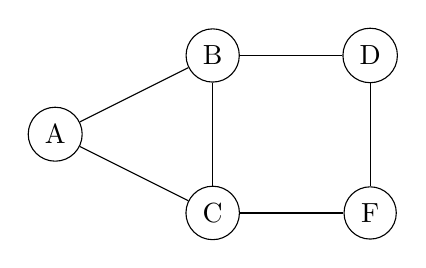
\begin{tikzpicture}[scale=2, rotate=90]
        % Nodes
        \node[circle, draw] (A) at (-0.5, 2) {A};
        \node[circle, draw] (B) at (0, 1) {B};
        \node[circle, draw] (C) at (-1, 1) {C};
        \node[circle, draw] (D) at (0, 0) {D};
        \node[circle, draw] (F) at (-1, 0) {F};
    
        % Edges
        \draw (A) -- (B);
        \draw (A) -- (C);
        \draw (B) -- (C);
        \draw (B) -- (D);
        \draw (C) -- (F);
        \draw (D) -- (F);
        \draw (F) -- (C);
    \end{tikzpicture}
    \caption{Beispiel eines Graphen}
    \label{fig:graph-ex}
\end{figure}
Der Graph in \cref{fig:graph-ex} besteht aus folgenden Komponenten:
\begin{itemize}
    \item Knoten $V=\lrc{A,B,C,D,F}$
    \item Kanten $E=\lrc{\lrc{A,B},\lrc{A,C},\lrc{B,C},\lrc{B,D},\lrc{C,F},\lrc{D,F}}$
\end{itemize}
\subsection{Wege und Kreise in Graphen}
Ein \tib{Weg} oder ein \tib{Spaziergang} in einem Graphen $G=(V,E)$ besteht aus einer Folge benachbarter Knoten, die miteinander verbunden werden. Ein Beispiel eines Wegs im Graph aus \cref{fig:graph-ex} wäre: $A,B,C,F,D$ (s. \cref{fig:graph-ex-weg}). 

\begin{figure}[H]
    \centering
    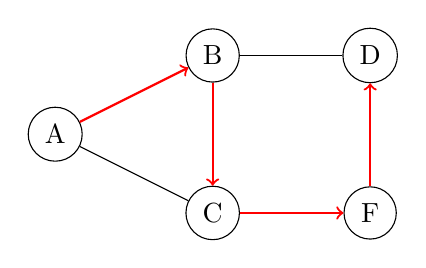
\begin{tikzpicture}[scale=2, rotate=90]
        % Nodes
        \node[circle, draw] (A) at (-0.5, 2) {A};
        \node[circle, draw] (B) at (0, 1) {B};
        \node[circle, draw] (C) at (-1, 1) {C};
        \node[circle, draw] (D) at (0, 0) {D};
        \node[circle, draw] (F) at (-1, 0) {F};
    
        % Edges
        \draw[->, thick, red] (A) -- (B);
        \draw (A) -- (C);
        \draw[->, thick, red] (B) -- (C);
        \draw (B) -- (D);
        \draw[->, thick, red] (C) -- (F);
        \draw[->, thick, red] (F) -- (D);
    \end{tikzpicture}
    \caption{Beispiel eines Wegs entlang eines Graphen.}
    \label{fig:graph-ex-weg}
\end{figure}

Wir sagen dem ersten und letzten Knoten in diesem Weg ($A$ und $D$) \tib{Endknoten} und wir nennen den Weg einen \tib{Kreis}, wenn die Endknoten gleich sind (z.B. $A,C,F,D,B,A$). Eine spezielle Art von Kreisen ist ein \tib{einfacher Kreis}, bei welchem ausser dem Endknoten kein anderer Knoten zweimal vorkommt.

Darüber hinaus gibt es weitere, spezielle Wege in Graphen:

Ein \tib{Euler'scher Weg} ist ein Weg, der alle Kanten eines Graphen genau einmal durchläuft. Graphen, die einen solchen Weg besitzen, nennen wir \tib{Euler'sche Graphen}.

Der berühmte Schweizer Mathematiker Leonhard Euler soll im Jahre 1736 die Stadt Königsberg besucht haben. Königsberg war damals die Hauptstadt der deutschen Provinz Ostpreussen. Seit dem Jahre 1946 gehört die Stadt zu Russland und wurde in \textit{Kaliningrad} unbenannt. In \cref{fig:stadtplanCrop} sehen Sie den für uns relevanten Ausschnitt eines Stadtplans des damaligen Königsbergs.
\begin{figure}[H]
    \centering
\begin{subfigure}{.4\textwidth}
    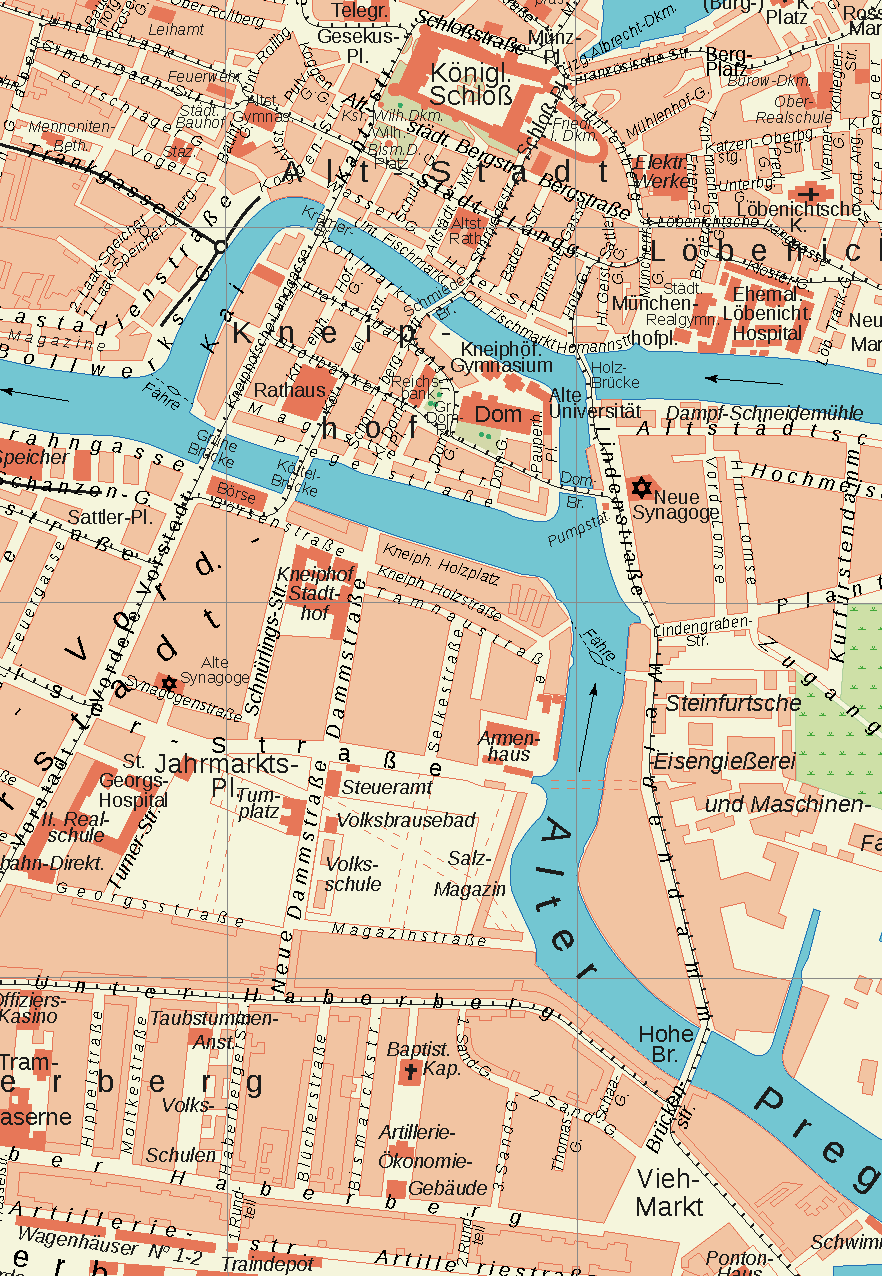
\includegraphics[width=\textwidth]{GrundlagenInfo/02_Graphen/AbstraktionDurchGraphen/Figures/StadplanCrop.pdf}
    \caption{Originaler Stadtplan}
    \label{fig:stadtplanCrop}
\end{subfigure}
\begin{subfigure}{.4\textwidth}
\centering
    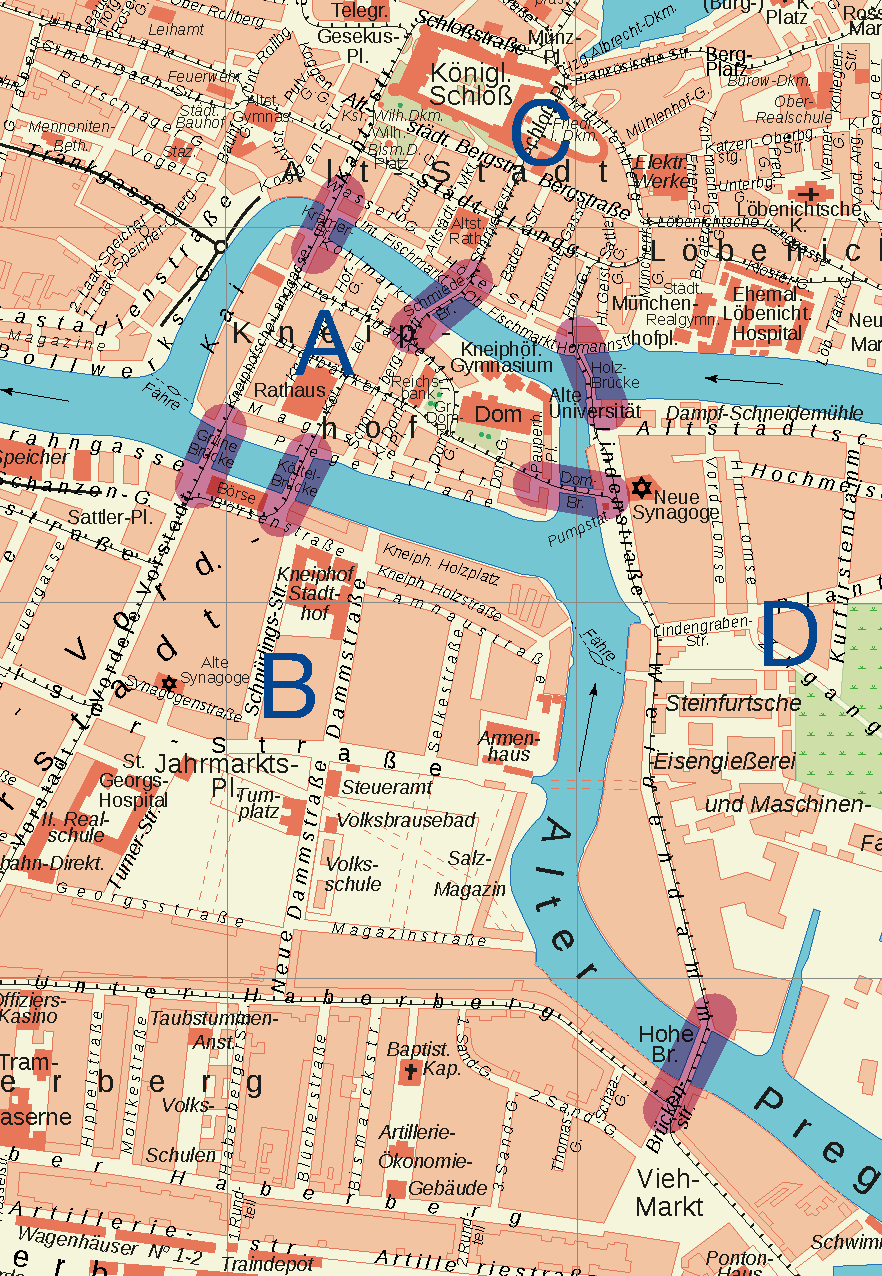
\includegraphics[width=\textwidth]{GrundlagenInfo/02_Graphen/AbstraktionDurchGraphen/Figures/StadplanCropMitBuchstaben.pdf}
    \caption{die vier Stadtteile $A, B, C$ und $D$ von Königsberg verbunden durch sieben Brücken}
    \label{fig:stadtplanCropMitBuchstaben}
\end{subfigure}
\caption{Ausschnitt aus einem Stadtplan des damaligen Königsbergs}
\end{figure}
\noindent
In \cref{fig:stadtplanCropMitBuchstaben} haben wir die vier verschiedenen Stadtteile Kneiphof ($A$), Vorstadt ($B$), Alt-Stadt ($C$) und Lomse ($D$) sowie die sieben Brücken zwischen ihnen hervorgehoben. Die Stadtteile werden von dem Fluss \textit{Pregel} von einander getrennt.

Der Legende nach kursierte unter den Spaziergängerinnen und Spaziergängern von Königsberg damals die folgende Frage, welche heute als \tib{Königsberger Brückenproblem} bekannt ist:
\begin{myexercise}[Königsberger Brückenproblem]\label{myBox:Problem}
Gibt es einen Weg durch Königsberg, bei dem man alle sieben Brücken \textbf{genau einmal} überquert, und wenn ja, ist auch ein Rundweg möglich, bei dem man wieder zum Ausgangspunkt gelangt?    
\end{myexercise}
\noindent
Euler realisierte vermutlich, dass es keine Rolle spielt, wie sich eine Spaziergängerin innerhalb eines Stadtteils bewegt. Relevant sind lediglich die Übergänge zwischen den Stadtteilen über die Brücken. Vermutlich abstrahierte er das Problem durch eine Skizze wie in \cref{fig:skizze}.

\begin{figure}[H]
    \centering
    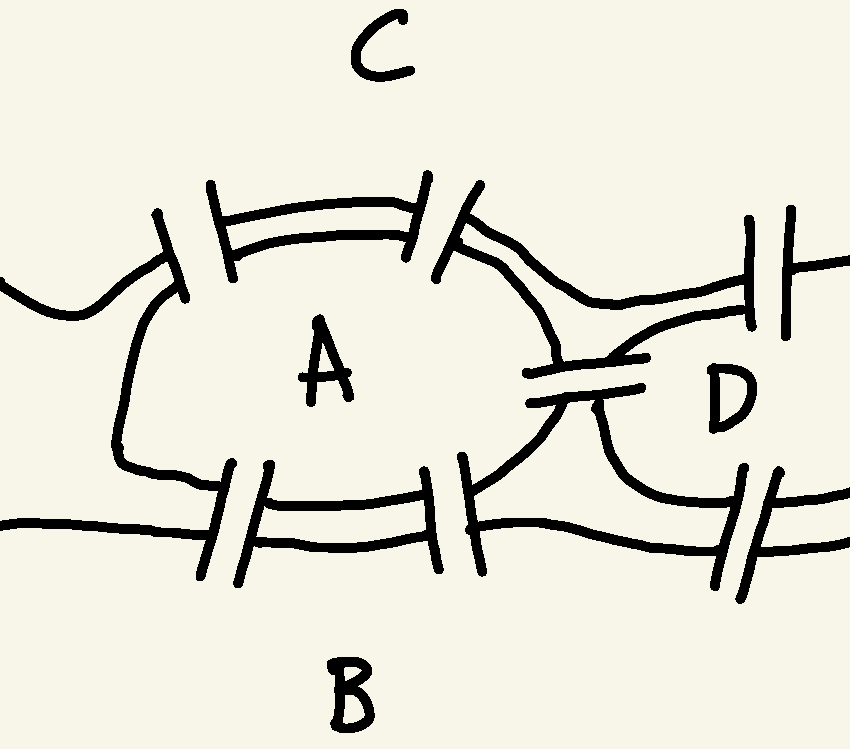
\includegraphics[width=0.3\textwidth]{GrundlagenInfo/02_Graphen/AbstraktionDurchGraphen/Figures/vonHandCrop.pdf}
    \caption{abstrakte Skizze von Königsberg}
    \label{fig:skizze}
\end{figure}

Selbst diese Skizze kann noch weiter abstrahiert werden, ohne dass wir relevante Informationen für das Königsberger Brückenproblem verlieren. Beispielsweise brauchen wir den Fluss nicht darzustellen. Dabei könnte man zur Abstraktion in \cref{subfig:graph} gelangen.

%% Aufgabenblatt %%
\begin{figure}[H]
\centering

\begin{subfigure}[b]{0.4\textwidth}
\centering
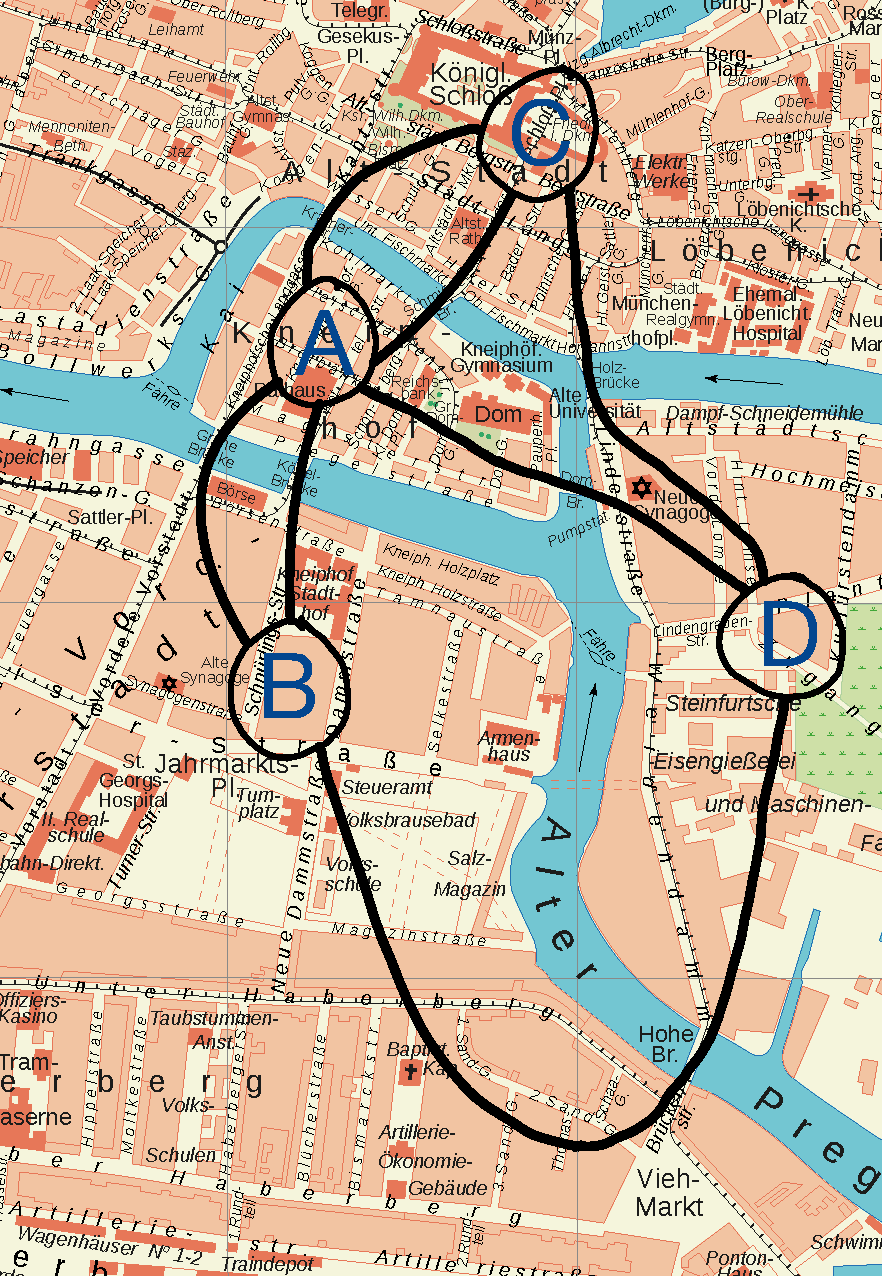
\includegraphics[width=0.9\textwidth]{GrundlagenInfo/02_Graphen/AbstraktionDurchGraphen/Figures/GraphAufStadtplan.pdf}
\caption{Stadtplan}
\end{subfigure}
\hfill
\begin{subfigure}[b]{0.4\textwidth}
\centering
\resizebox{0.7\textwidth}{!}{
\begin{tikzpicture}[shorten >=1pt,auto,node distance=3cm, semithick, scale=0.25]
  \node[state] (A)              {$A$};
  \node[state] (B) [below of=A] {$B$};
  \node[state] (C) [above of=A] {$C$};
  \node[state] (D) [right of=A] {$D$};

  \path (A) edge [bend right] node {} (B)
        (A) edge [bend left] node {} (B)
        (A) edge [bend right] node {} (C)
        (A) edge [bend left] node {} (C)
        (A) edge node {} (D)
        (B) edge node {} (D)
        (C) edge node {} (D);
\end{tikzpicture}
}
\caption{Darstellung als Graph}
\label{subfig:graph}
\end{subfigure}
\caption{Modellierung des Königsberger Brückenproblems durch einen Graphen mit vier Knoten und sieben Kanten}
\label{fig:EulerGraph}
\end{figure}

Die schematische Darstellung in \cref{subfig:graph} ist lediglich ein Modell der eigentlichen Situation in Königsberg. Allerdings enthält dieses Modell sämtliche für das Problem relevanten Teile und lässt alle nicht relevanten Teile geschickt weg. Das Modell stellt also eine hervorragende Abstraktion des Problems dar. Eine solche Art der Abstraktion wie in \cref{subfig:graph}  wird \tib{Graph} genannt.



Ein \tib{Hamilton'scher Weg} ist ein einfacher Weg zwischen zwei Knoten eines Graphen, bei dem alle Knoten des Graphen enthalten sind.

\begin{myexercise}
Suchen Sie Euler'sche Wege/Kreise und Hamilton'sche Wege/Kreise im Graph aus \cref{fig:graph-ex}.
\begin{myanswer}
Der Graph besitzt nur Euler'schen Wege, aber keine Kreise. Ein möglicher Euler'scher Weg ist in \cref{fig:graph-ex-weg-eul-1} abgebildet.
\begin{figure}[H]
    \centering
    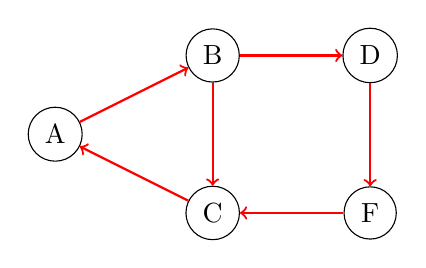
\begin{tikzpicture}[scale=2, rotate=90]
        % Nodes
        \node[circle, draw] (A) at (-0.5, 2) {A};
        \node[circle, draw] (B) at (0, 1) {B};
        \node[circle, draw] (C) at (-1, 1) {C};
        \node[circle, draw] (D) at (0, 0) {D};
        \node[circle, draw] (F) at (-1, 0) {F};
    
        % Edges
        \draw[->, thick, red] (A) -- (B);
        \draw[->, thick, red] (C) -- (A);
        \draw[->, thick, red] (B) -- (C);
        \draw[->, thick, red] (B) -- (D);
        \draw[->, thick, red] (F) -- (C);
        \draw[->, thick, red] (D) -- (F);
    \end{tikzpicture}
    \caption{Euler'scher Weg 1 $B,D,F,C,A,B,C$ entlang des Graphen aus \cref{fig:graph-ex}}
    \label{fig:graph-ex-weg-eul-1}
\end{figure}
\end{myanswer}
Der Graph besitzt viele Hamilton'sche Wege und Kreise, z.B. $A,B,D,F,C$.
\end{myexercise}

\begin{mychallenge}
Versuchen Sie, eine allgemeine Regel zu finden, um für beliebige Graphen zu bestimmen, ob es Euler'schen Wege und Kreise gibt oder nicht.
\begin{myanswer}
Ein ungerichteter Graph besitzt genau dann einen Euler'schen Weg, wenn die folgenden Bedingungen erfüllt sind:
\begin{itemize}
\item Der Graph ist \textbf{zusammenhängend}, wenn man die isolierten Knoten ignoriert (d.h. man kann von jedem Knoten zu jedem anderen Knoten gelangen).
\item \textbf{Genau zwei Knoten} haben eine \textbf{ungerade Anzahl von Kanten} (ungeraden Grad), oder es gibt \textbf{keinen Knoten mit ungeradem Grad}.
\item Falls kein Knoten ungeraden Grad hat, dann besitzt der Graph einen Euler'schen Kreis (geschlossener Eulerweg).
\item Falls genau zwei Knoten ungeraden Grad haben, dann besitzt der Graph einen Euler'schen Weg, der an einem der Knoten mit ungeradem Grad beginnt und am anderen endet.
\end{itemize}
\end{myanswer}
\end{mychallenge}
\subsection{Nachbarschafts-Matrizen}
Bisher haben wir Graphen lediglich als Zeichnung sowie durch die Beschreibung deren Kanten und Knoten zu beschreiben gelernt. Wir können Grahen jedoch auch als Nachbarschafts-Matrize schreiben.


\begin{figure}[H]
\centering

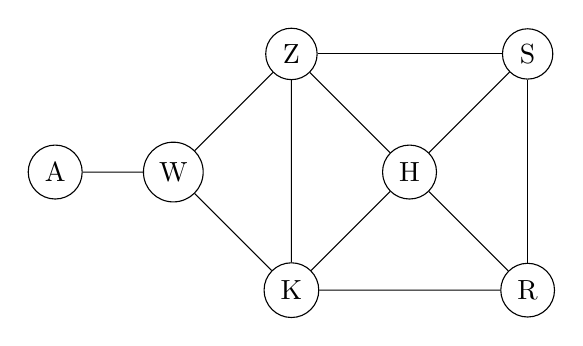
\begin{tikzpicture}[rotate=180, scale=1.5]
    % Nodes
    \node[circle, draw] (R) at (0, 2) {R};
    \node[circle, draw] (S) at (0, 0) {S};
    \node[circle, draw] (K) at (2, 2) {K};
    \node[circle, draw] (Z) at (2, 0) {Z};
    \node[circle, draw] (H) at (1, 1) {H};
    \node[circle, draw] (W) at (3, 1) {W};
    \node[circle, draw] (A) at (4, 1) {A};

    % Edges
    \draw (R) -- (K);
    \draw (R) -- (S);
    \draw (R) -- (H);
    \draw (S) -- (H);
    \draw (S) -- (Z);
    \draw (K) -- (H);
    \draw (K) -- (Z);
    \draw (Z) -- (H);
    \draw (K) -- (W);
    \draw (Z) -- (W);
    \draw (W) -- (A);
\end{tikzpicture}
\caption{Ungerichteter Graph}
\label{fig:ex-graph-2}
\end{figure}

Die \textbf{Nachbarschaftsmatrix} bezeichnet eines Graphs gibt Aufschluss darüber, welche Knoten mit welchen anderen Knoten verbunden sind. \cref{tab:nachbarschaft-ex-1} zeigt die Nachbarschaftsmatrix für den Graphen aus \cref{fig:ex-graph-2}.

\begin{table}[H]
\centering
\begin{tabular}{c||c|c|c|c|c|c|c}
  & R & S & H & K & Z & W & A \\ \midrule
R & 0 & 1 & 1 & 1 & 0 & 0 & 0\\ \hline
S & 1 & 0 & 1 & 0 & 1 & 0 & 0\\ \hline
H & 1 & 1 & 0 & 1 & 1 & 0 & 0\\ \hline
K & 1 & 0 & 1 & 0 & 1 & 1 & 0\\ \hline
Z & 0 & 1 & 1 & 1 & 0 & 1 & 0\\ \hline
W & 0 & 0 & 0 & 1 & 1 & 0 & 1\\ \hline
A & 0 & 0 & 0 & 0 & 0 & 1 & 0\\ 
\end{tabular}
\caption{Nachbarschaftsmatrix des Graphen aus \cref{fig:ex-graph-2}}
\label{tab:nachbarschaft-ex-1}
\end{table}


\subsection{Gewichtete Graphen}
Bisher haben wir uns lediglich ungerichtete Graphen angeschaut, d.h., Graphen bei denen die Kanten keine spezielle Richtung aufweisen. Graphen könenn allerdings in vielen Fällen auch gerichtet sein, beispielsweise, wenn es darum geht, zu beschreiben, wer wen kennt.


\begin{figure}[H]
\centering
\begin{tikzpicture}[
    ->, % Arrow style
    node distance=2cm and 2cm, % Distance between nodes
    every node/.style={circle, draw, minimum size=1cm}, % Node style
    thick % Line thickness
]

% Nodes
\node (Wilson) {Wilson};
\node (Sofia) [above left=of Wilson] {Sofia};
\node (Laura) [above right=of Wilson] {Laura};
\node (Elia) [below left=of Wilson] {Elia};
\node (Igor) [below right=of Wilson] {Igor};
\node (Lara) [below=of Wilson] {Lara};

% Edges
\draw (Sofia) -- (Wilson);
\draw (Laura) -- (Wilson);
\draw (Elia) -- (Wilson);
\draw (Igor) -- (Wilson);
\draw (Lara) -- (Wilson);

\draw (Sofia) edge[bend left=10] (Laura);
\draw (Laura) edge[bend left=10] (Sofia);
\draw (Laura) -- (Igor);
\draw (Igor) -- (Lara);
\draw (Elia) edge[bend left=10] (Lara);
\draw (Lara) edge[bend left=10] (Elia);
\draw (Elia) edge[bend left=10] (Sofia);
\draw (Sofia) edge[bend left=10] (Elia);
\draw[out=310, in=320, looseness=1.6] (Laura) to (Lara);
\draw[out=340, in=290, looseness=1.7] (Lara) to (Laura);
\draw[out=110, in=160, looseness=2.3] (Elia) to (Laura);

\end{tikzpicture}
\caption{Gerichter Graph, um Freundschaften darzustellen}.
\end{figure}

\begin{table}[H]
\centering
\begin{tabular}{c||c|c|c|c|c|c}
        & Sofia & Laura & Igor & Wilson & Elia & Lara \\ \midrule
Sofia     & 0 & 1 & 0 & 1 & 1 & 0 \\ \hline
Laura & 1 & 0 & 1 & 1 & 0 & 1 \\ \hline
Igor     & 0 & 0 & 0 & 1 & 0 & 1 \\ \hline
Wilson    & 0 & 0 & 0 & 0 & 0 & 0 \\ \hline
Elia    & 1 & 1 & 0 & 1 & 0 & 1 \\ \hline
Lara     & 0 & 1 & 0 & 1 & 1 & 0 \\
\end{tabular}
\end{table}

\subsection{Bäume}
Definitionen
\begin{itemize}
    \item \emoji{deciduous-tree} Ein Graph heisst \textbf{Baum}, wenn er \textbf{zusammenhängend} und \textbf{kreisfrei} ist.
    \item \emoji{maple-leaf} Knoten mit Grad 1 = \textbf{Blätter} eines Baums
\end{itemize}

\begin{myexercise}
Welche dieser drei Graphen sind Bäume? Weshalb (nicht)?
\begin{figure}[H]
    \centering
    \begin{tabular}{c|c|c}
        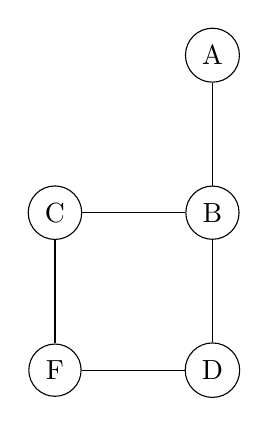
\begin{tikzpicture}[scale=2]
            % Nodes
            \node[circle, draw] (A) at (0, 2) {A};
            \node[circle, draw] (B) at (0, 1) {B};
            \node[circle, draw] (C) at (-1, 1) {C};
            \node[circle, draw] (D) at (0, 0) {D};
            \node[circle, draw] (F) at (-1, 0) {F};
        
            % Edges
            \draw (A) -- (B);
%            \draw (A) -- (C);
            \draw (B) -- (C);
            \draw (B) -- (D);
            \draw (C) -- (F);
            \draw (D) -- (F);
            \draw (F) -- (C);
        \end{tikzpicture}&
        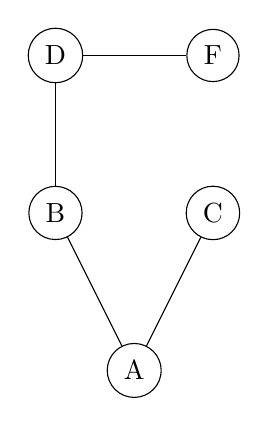
\begin{tikzpicture}[scale=2, rotate=180]
            % Nodes
            \node[circle, draw] (A) at (-0.5, 2) {A};
            \node[circle, draw] (B) at (0, 1) {B};
            \node[circle, draw] (C) at (-1, 1) {C};
            \node[circle, draw] (D) at (0, 0) {D};
            \node[circle, draw] (F) at (-1, 0) {F};
        
            % Edges
            \draw (A) -- (B);
            \draw (A) -- (C);
%            \draw (B) -- (C);
            \draw (B) -- (D);
%            \draw (C) -- (F);
            \draw (D) -- (F);
%            \draw (F) -- (C);
        \end{tikzpicture}&
        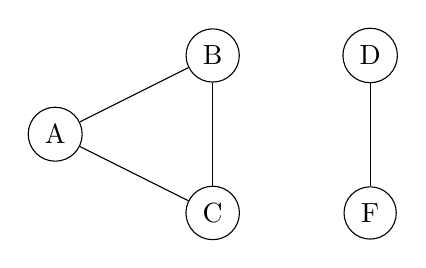
\begin{tikzpicture}[scale=2, rotate=90]
            % Nodes
            \node[circle, draw] (A) at (-0.5, 2) {A};
            \node[circle, draw] (B) at (0, 1) {B};
            \node[circle, draw] (C) at (-1, 1) {C};
            \node[circle, draw] (D) at (0, 0) {D};
            \node[circle, draw] (F) at (-1, 0) {F};
        
            % Edges
            \draw (A) -- (B);
            \draw (A) -- (C);
            \draw (B) -- (C);
%            \draw (B) -- (D);
%            \draw (C) -- (F);
            \draw (D) -- (F);
%            \draw (F) -- (C);
        \end{tikzpicture}\\
        \end{tabular}
%    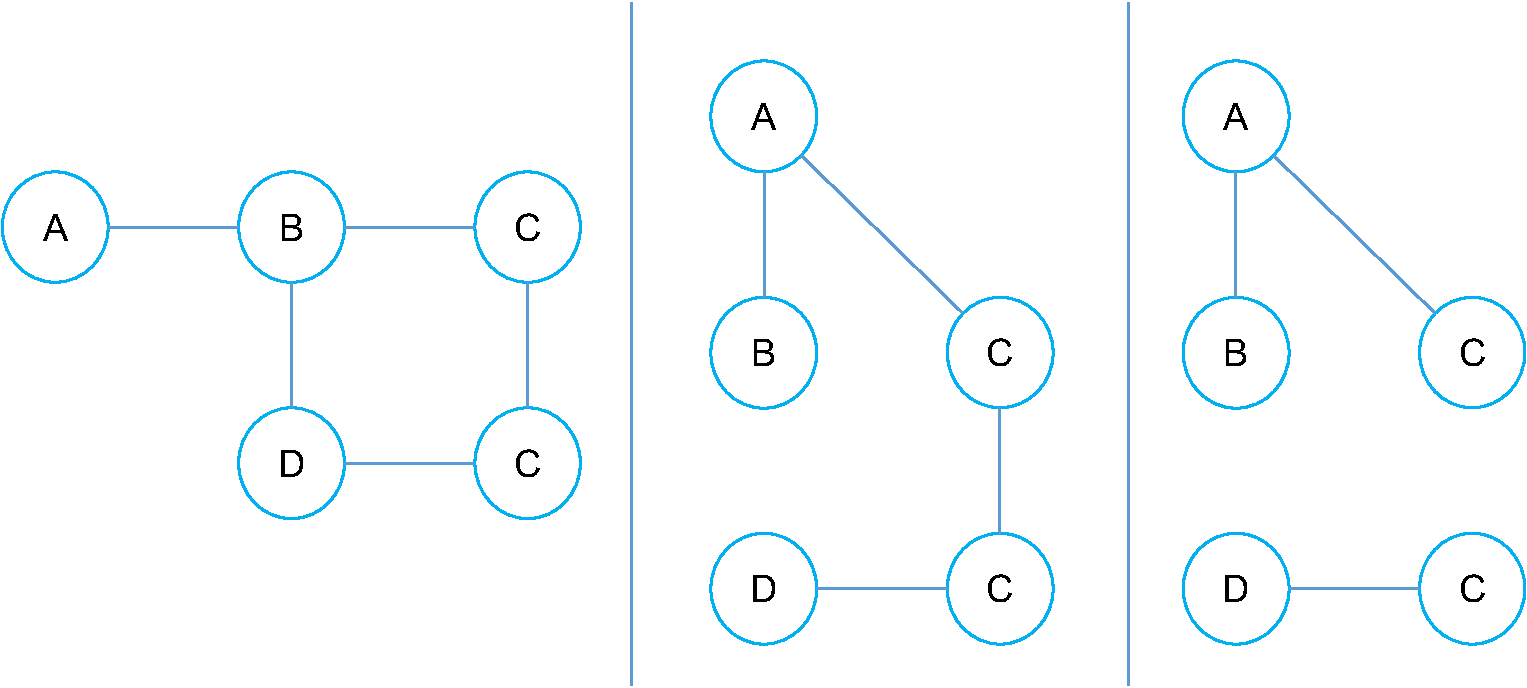
\includegraphics[keepaspectratio, width=.8\linewidth]{GrundlagenInfo/02_Graphen/Figures/graphen-baeume.pdf}
\end{figure}
\begin{myanswer}
Nur der zweite Graph ist ein Baum. Der erste Graph ist nicht kreisfrei und der dritte ist nicht zusammenhängend.
\end{myanswer}
\end{myexercise}


\begin{figure}[H]
    \centering
%    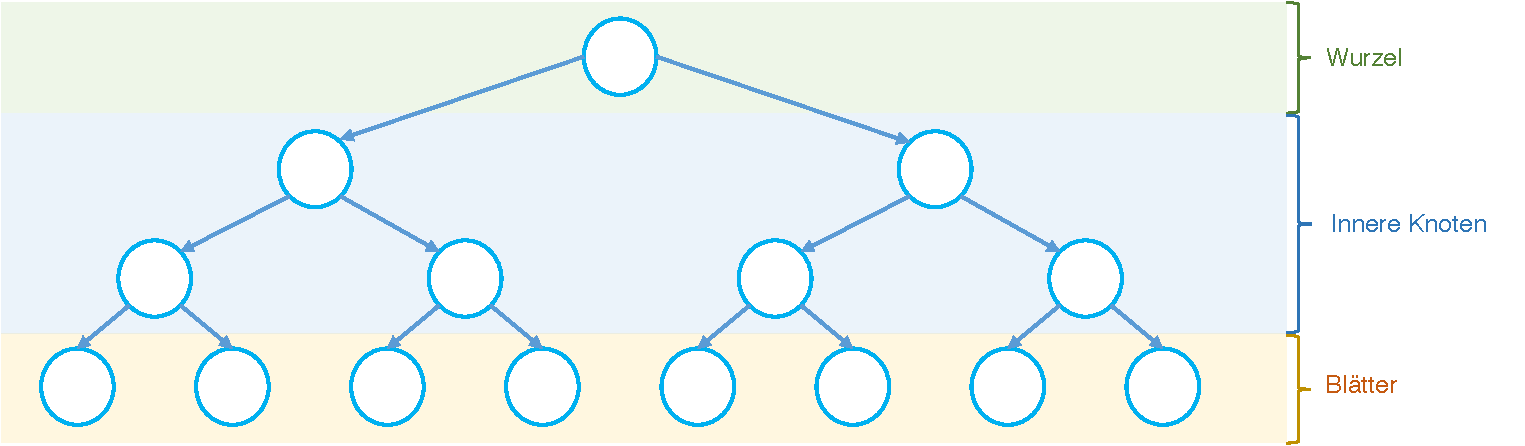
\includegraphics[keepaspectratio, width=\linewidth]{GrundlagenInfo/02_Graphen/Figures/binary-tree.pdf}
   

   \begin{tikzpicture}[
     every node/.style={circle, draw, minimum size=8mm}, % Define size of the nodes
     edge from parent/.style={draw, -latex},
     level distance=20mm, % Adjust spacing between levels and siblings
     level 1/.style={sibling distance=40mm},   % Sibling distance for level 1
     level 2/.style={sibling distance=20mm},   % Sibling distance for level 2
   ]
   
     % Background rectangles with exact positioning
     \begin{scope}[on background layer]
       \fill[red!20] (-5,0) rectangle (5,2);  % Root level background
       \fill[green!20] (-5,-2) rectangle (5,0); % Inner nodes background
       \fill[blue!20] (-5,-4) rectangle (5,-2);  % Leaf nodes background
     \end{scope}
   
     % Nodes with precise coordinates
     \node at (0, 1) (root) {} % Root node position
       child { node (innerL) {}
         child { node (leafL) {} }
         child { node (leafR) {} }
       }
       child { node (innerR) {}
         child { node  {} }
         child { node  {} }
       };
   
     % Braces for annotations
     \draw[decorate,decoration={brace,amplitude=10pt}] (5,2) -- (5,0) node[draw=none,anchor=west,midway,xshift=10pt] {Wurzel};
     \draw[decorate,decoration={brace,amplitude=10pt}] (5,0) -- (5,-2) node[draw=none,anchor=west,midway,xshift=10pt] {Innere Knoten};
     \draw[decorate,decoration={brace,amplitude=10pt}] (5,-2) -- (5,-4) node[draw=none,anchor=west,midway,xshift=10pt] {Blätter};
   
   \end{tikzpicture}
  
   
   
\end{figure}
\begin{itemize}
    \item \textbf{Wurzel} = Knoten mit Eingangs-Grad 0
    \item \textbf{Blätter} = Knoten mit Ausgangs-Grad 0
    \item \textbf{Innere Knoten} = Alle anderen Knoten (weder Blätter noch Wurzel)
    \item Das Beispiel oben ist ein \textbf{gewurzelter Baum}: Es gibt eine einzige Wurzel, von der aus alle Knoten über gerichtete Kanten erreichbar sind
\end{itemize}

\subsection{Kürzeste Wege}
Eine der wichtigsten und schwierigsten Aufgaben in einem Netzwerk ist es, den kürzesten Weg von A nach B zu finden.

\begin{mycaution}
Dieser Abschnitt befindet sich noch im Aufbau und wird zu einem späteren Zeitpunkt vervollständigt.
\end{mycaution}
\newpage
